% =====================================================================
% CAPÍTULO 5: RESULTADOS (piso de rodadas)
% Substitui o resultados.tex do v1, que fica fora do main.tex como material.
% Fontes dos números da Seção~\ref{sec:res-calibracao}:
%   build/reduced_rounds/floor_v2/contador_zero_corpus_en/<algo>_floor/piso.csv
%   (estudo principal) e todos os piso.csv de floor_v2/ para a taxa de falso
%   positivo, sem Grain e sem os modelos fora da dissertação (ResNet, CNN 2D,
%   híbrido), levantados em 19/10/2026 e atualizados em 25/10/2026.
% =====================================================================

\chapter{Resultados}
\label{cap:resultados}

Este capítulo apresenta os resultados dos experimentos descritos no Capítulo~\ref{cap:metodologia}. A Seção~\ref{sec:res-calibracao} verifica se o critério de detecção se comporta como esperado nos próprios dados do experimento. A Seção~\ref{sec:res-isolado} trata do criptograma isolado, e a Seção~\ref{sec:res-piso} mede o piso de rodadas com pares de mensagens consecutivas, que é o resultado principal do trabalho. A Seção~\ref{sec:res-robustez} testa se esse piso muda quando se muda a forma de medir, e a Seção~\ref{sec:res-sintese} resume os resultados. A interpretação dos resultados e a comparação com a literatura ficam para o Capítulo~\ref{cap:discussao}.

\section{Calibração do critério de detecção}
\label{sec:res-calibracao}

Antes de medir qualquer piso, é preciso saber se o critério de detecção acusa sinal onde ele não existe e se acusa sinal onde ele certamente existe. Nos três algoritmos, nenhuma célula do braço de controle aleatório foi detectada com a tag incluída, e, sem ela, uma foi detectada, sem formar piso, nenhuma célula com número de rodadas próximo da especificação foi detectada, e todas as células com uma e com duas rodadas foram detectadas, com F1 de pelo menos 0,99.

Os números desta seção vêm do estudo principal, com texto em claro extraído de livros do Project Gutenberg, contador de nonce começando do zero em cada dispositivo, 300 chaves com 100 pares cada e 60 chaves reservadas para teste, o que dá 12\,000 amostras de teste por configuração, 6\,000 de cada classe. Cada número de rodadas é avaliado por três classificadores (regressão logística, Random Forest e XGBoost) e três tamanhos de bolsa (1, 10 e 100 pares do mesmo dispositivo por decisão), o que dá nove células por rodada. A bolsa junta a opinião do classificador sobre vários pares do mesmo dispositivo numa decisão só. Para cada par, a probabilidade $p$ de ser cifra, dada pelo classificador, é convertida em log-odds~\cite{Cox1958}, $\ln\big(p/(1-p)\big)$, um valor que é zero quando o classificador não tem preferência ($p = 0{,}5$), positivo quando ele aponta a cifra e negativo quando aponta o aleatório. A decisão da bolsa é o sinal da média dos log-odds dos seus 10 ou 100 pares. A média é feita nessa escala, e não sobre as probabilidades, porque nela a evidência de pares independentes se soma~\cite{Good1950}. Como os pares de uma bolsa compartilham a chave, a média é usada aqui como regra de agregação, sem supor essa independência.

O p-valor de cada célula mede a chance de um F1 tão alto aparecer se o classificador não tivesse sinal nenhum, e é calculado a partir da variação do F1 nas reamostragens por chave descritas no fim desta seção. Cada estudo avalia várias rodadas, nos dois braços, em nove células por rodada, ou seja, mais de cem testes ao mesmo tempo, e com tantos testes alguns dariam p-valor abaixo de 0,05 só por acaso. Para controlar esse efeito foi usada a correção de Benjamini-Hochberg~\cite{Benjamini1995FDR}, que ordena os p-valores do menor para o maior e compara cada um com um limite proporcional à sua posição na ordem, de modo que, entre todas as células declaradas significativas, a proporção esperada de falsos positivos fique abaixo de 5\%. Ela foi preferida à correção de Bonferroni porque esta controla a chance de haver um único falso positivo entre todos os testes e, com mais de cem deles, fica tão rigorosa que esconderia os sinais fracos que existem perto do piso. Uma célula conta como detectada quando sobrevive a essa correção e fica acima do maior F1 observado na faixa de controle para o mesmo classificador e tamanho de bolsa, e um piso só é declarado quando todas as rodadas abaixo dele também são detectadas, conforme definido no Capítulo~\ref{cap:metodologia}.

O controle negativo é o braço aleatório, em que o mesmo algoritmo, com as mesmas chaves e os mesmos nonces, cifra texto em claro aleatório, formado por bytes sorteados, no lugar do texto dos livros. Nos três algoritmos, cada bloco cifrado é o bloco de texto em claro somado (XOR) a um valor que não depende desse bloco, então, quando o texto é aleatório, a parte cifrada de cada criptograma também é aleatória, e o mesmo vale para o XOR dos dois criptogramas do par, por mais fraca que seja a cifra. Na parte cifrada, qualquer detecção nesse braço é, portanto, falso positivo por construção, mas a tag não tem essa garantia, e uma detecção com a tag incluída pode ser sinal dela. Por isso, o controle foi feito com a tag e sem ela. Com a tag incluída, como no braço de texto, nenhuma das 180 células do braço aleatório do estudo principal teve p-valor abaixo de 0,05, nem antes da correção. Sem a tag, só com os 64 bytes de texto cifrado, uma das 180 células foi detectada, no GIFT-COFB com cinco rodadas, com o Random Forest e bolsas de 100 pares. Como, sem a tag, o braço aleatório não tem sinal possível, essa célula é um falso positivo do procedimento. Ela não formou piso, já que nenhuma rodada abaixo dela foi detectada nesse braço, e nenhum dos três algoritmos teve piso no braço aleatório, com a tag ou sem ela.

A faixa de controle é o segundo controle negativo. Ela reúne as rodadas a partir da metade da especificação (8 e 12 no Ascon-AEAD128, 20 e 40 no GIFT-COFB, 8 e 11 no Schwaemm256-128), em que a diferença entre os nonces do par já passou por muitas rodadas e não se espera sinal. Diferente do braço aleatório, ela usa o texto real dos livros, então mede quanto um detector oscila por acaso nas mesmas condições do experimento. Para cada combinação de classificador e tamanho de bolsa, o maior F1 observado nessa faixa vira o teto do critério, para que uma rodada mais baixa conte como detectada, ela precisa ficar acima desse valor. A ausência de sinal na faixa é uma suposição, e não uma garantia como no braço aleatório. Se ela estiver errada, o teto sobe e o critério fica mais rigoroso. Nenhuma das 54 células da faixa passou pela correção de Benjamini-Hochberg, e os tetos ficaram entre 0,499 e 0,541 no Ascon-AEAD128, entre 0,450 e 0,574 no GIFT-COFB e entre 0,458 e 0,525 no Schwaemm256-128, com os valores mais altos nas bolsas de 100, que têm menos decisões e por isso variam mais.

O controle positivo são as rodadas mais baixas, em que a diferença entre os nonces do par ainda não se espalhou pelo estado e o sinal é forte. Com uma e com duas rodadas, as 54 células do braço de texto foram detectadas nos três algoritmos, com F1 entre 0,993 e 1,000.

\begin{table}[htb]
\centering
\caption{Calibração do critério de detecção nos três algoritmos.}
\label{tab:res-calibracao}
\small
\setlength{\tabcolsep}{2.5pt}
\begin{tabular}{lcccccc}
\toprule
 & \multicolumn{3}{c}{braço aleatório} & \multicolumn{2}{c}{faixa de controle} & \\
\cmidrule(lr){2-4}\cmidrule(lr){5-6}
 & & \multicolumn{2}{c}{detectadas} & & & \\
\cmidrule(lr){3-4}
Algoritmo & células & com a tag & sem a tag & rodadas & detectadas & F1 com 1 e 2 rodadas \\
\midrule
Ascon-AEAD128   & 63 & 0 & 0 & 8 e 12  & 0 de 18 & 0,995 a 1,000 \\
GIFT-COFB       & 63 & 0 & 1 & 20 e 40 & 0 de 18 & 0,995 a 1,000 \\
Schwaemm256-128 & 54 & 0 & 0 & 8 e 11  & 0 de 18 & 0,993 a 1,000 \\
\bottomrule
\end{tabular}
\end{table}

A Tabela~\ref{tab:res-calibracao} reúne os três controles. Com a tag incluída, nenhum dos três algoritmos teve célula detectada nos controles negativos, e, sem a tag, o GIFT-COFB teve uma. No braço aleatório, foram avaliadas 63 células no Ascon-AEAD128, 63 no GIFT-COFB e 54 no Schwaemm256-128, e, com a tag incluída, nenhuma foi detectada; na faixa de controle, nenhuma das 18 células de cada algoritmo foi detectada. No controle positivo, ao contrário, as rodadas 1 e 2 tiveram F1 entre 0,993 e 1,000 nos três. Esse resultado é relevante porque mostra que o critério não produz piso onde não existe sinal e produz detecções onde o sinal é forte. É com base nessas duas propriedades que o piso, situado entre esses dois extremos, na rodada 3 do Ascon-AEAD128 e do GIFT-COFB e na rodada 2 do Schwaemm256-128, pode ser atribuído à cifra reduzida, e não a um artefato do instrumento de medida.

Somando todos os estudos de piso realizados com os três algoritmos, inclusive as variações das Seções~\ref{sec:res-isolado}, \ref{sec:res-piso} e~\ref{sec:res-robustez}, o braço aleatório teve 3\,804 células, todas com a tag incluída. Antes de qualquer correção, 1,9\% delas tiveram p-valor abaixo de 0,05, próximo dos 2,5\% esperados ao acaso, já que, ao tomar o p-valor como 1 quando o F1 fica abaixo de 0,50, o teste é, na prática, unilateral. Depois da correção de Benjamini-Hochberg restaram 0,37\%, e depois do critério completo 0,26\%, o que corresponde a dez células, duas com a representação que junta os dois criptogramas ao XOR, uma com a MLP recebendo os dois criptogramas inteiros, uma com a MLP recebendo o XOR e seis no estudo com nonces a distância $k$ (Seção~\ref{sec:res-contador}). Nenhuma delas formou piso, porque em nenhum dos dez casos a rodada 1 do mesmo braço foi detectada. Como essas células incluem a tag, que pode carregar estrutura da finalização reduzida, não é possível afirmar que sejam falsos positivos, e elas não foram reanalisadas sem a tag.

A taxa de falso positivo do procedimento foi medida, então, onde não há sinal possível, no teste A/A descrito na Seção~\ref{sec:met-braco-aleatorio}, em que as duas classes são amostras do mesmo processo aleatório. Nas 20 réplicas, com nove células cada, 5 das 180 células (2,8\%) tiveram p-valor abaixo de 0,05, próximo dos 2,5\% esperados, e nenhuma passou pela correção de Benjamini-Hochberg. O F1 sem sinal nenhum chegou a 0,510 com bolsas de um par, a 0,537 com bolsas de 10 e a 0,600 com bolsas de 100, o que mostra quanto as bolsas de 100 oscilam por acaso e por que o teto da faixa de controle é calculado separadamente para cada tamanho de bolsa.

Nos números das próximas seções, o acaso corresponde a AUC de 0,50. No F1 macro, um classificador sem sinal fica perto de 0,50 quando divide as respostas entre as duas classes e em cerca de 0,33 quando responde sempre a mesma classe. Os intervalos de confiança são obtidos por \textit{bootstrap} com 1\,000 reamostragens por chave, e não por amostra, porque pares do mesmo dispositivo compartilham a chave e não são independentes. Por fim, um piso declarado indica que até aquele número de rodadas o algoritmo reduzido é separável de dados aleatórios por pelo menos um dos detectores avaliados, e a ausência de detecção acima dele não é evidência de segurança, apenas de que esses detectores, com essa quantidade de dados, não separam.

\section{Criptograma isolado}
\label{sec:res-isolado}

Esta seção verifica, com dois experimentos, se um criptograma isolado já permite reconhecer um algoritmo enfraquecido. Com criptogramas de 64~KB descritos por atributos estatísticos, nenhum classificador superou o acaso, com AUC entre 0,49 e 0,51, mesmo com os três algoritmos reduzidos a uma rodada. Com criptogramas de 80 bytes descritos pelos bits crus, o criptograma isolado passou a denunciar os algoritmos, mas só praticamente sem rodadas, com uma rodada no Ascon-AEAD128 e no GIFT-COFB e com duas, de forma marginal, no Schwaemm256-128.

\subsection{Criptograma de 64 KB com atributos estatísticos}
\label{sec:res-isolado-64k}

A tarefa deste experimento era a seguinte: o classificador recebia um criptograma e precisava dizer se ele tinha sido gerado pelo algoritmo ou se eram dados aleatórios do mesmo tamanho. Foram cifradas mensagens de 64~KB extraídas de livros do Project Gutenberg, com 300 chaves e 100 mensagens por chave, as mesmas para os três algoritmos, o que dá 30\,000 criptogramas por algoritmo e outras 30\,000 amostras aleatórias, separadas por chave em 240 chaves para treinamento e 60 para teste. Cada criptograma foi descrito pelos 641 atributos estatísticos da Seção~\ref{sec:met-atributos} e submetido aos três classificadores do estudo principal, com bolsas de 1, 10 e 100 mensagens.

Os três algoritmos foram reduzidos a uma rodada, nas duas fases no Ascon-AEAD128 e no Schwaemm256-128 e em todas as chamadas da cifra de bloco no GIFT-COFB. A Tabela~\ref{tab:res-isolado} traz, para cada algoritmo, o classificador de maior F1 por mensagem e a sua matriz de confusão.

\begin{table}[htb]
\centering
\caption{Melhor classificador por algoritmo com o criptograma isolado, com uma rodada.}
\label{tab:res-isolado}
\footnotesize
\setlength{\tabcolsep}{3pt}
\begin{tabular}{llccrrrr}
\toprule
Algoritmo & Melhor modelo & F1 (IC 95\%) & AUC & A$\to$A & A$\to$C & C$\to$A & C$\to$C \\
\midrule
Ascon-AEAD128 & RF & 0,504 [0,494; 0,514] & 0,502 & 3\,124 & 2\,876 & 3\,075 & 2\,925 \\
GIFT-COFB & Reg. log. & 0,503 [0,493; 0,512] & 0,500 & 3\,068 & 2\,932 & 3\,029 & 2\,971 \\
Schwaemm256-128 & XGBoost & 0,506 [0,497; 0,514] & 0,500 & 2\,967 & 3\,033 & 2\,899 & 3\,101 \\
\bottomrule
\end{tabular}
\par\smallskip\footnotesize Nota: A = aleatório e C = cifra, na forma classe verdadeira$\to$classe prevista, com bolsa de uma mensagem.
\end{table}

Nos três algoritmos, o melhor classificador ficou com F1 entre 0,503 e 0,506 e AUC entre 0,500 e 0,502, e as matrizes de confusão mostram os erros distribuídos de forma quase igual entre as duas classes, que é o padrão esperado de um classificador que não encontrou diferença entre elas. Em nenhum dos três algoritmos alguma das nove células passou pela correção de Benjamini-Hochberg, e o menor p-valor foi de 0,194. Por isso, nem o teto da faixa de controle nem o braço aleatório precisaram ser usados, já que não havia detecção a ser conferida.

Como uma cifra com uma rodada não é segura, o resultado indica que o problema estava no que o classificador observava, e não na força da cifra. Uma explicação possível é a diluição: a parte do criptograma que sai de um estado mal misturado fica no início da mensagem, e os atributos, calculados sobre os 65\,552 bytes do criptograma, não isolam essa região. O Schwaemm256-128 com uma rodada é compatível com essa hipótese, já que é separado dos dados aleatórios com F1 de 0,999 quando a mensagem tem 64 bytes e o classificador recebe os bits crus (Seção~\ref{sec:res-isolado-80b}), e fica no acaso quando o criptograma tem 64~KB e é descrito pelos atributos.

\subsection{Criptograma de 80 bytes com bits crus}
\label{sec:res-isolado-80b}

Essa observação orientou o desenho do segundo experimento, que mudou o que o classificador observa em dois pontos. Em vez dos 641 atributos estatísticos calculados sobre o criptograma inteiro, o classificador passou a receber os bits crus do criptograma, de modo que cada posição pudesse ser avaliada separadamente. E o criptograma foi reduzido a 80 bytes, 64 de texto cifrado e 16 de tag, o que concentra a análise no início da mensagem, logo depois da inicialização. Esse tamanho também é mais próximo do uso real da criptografia leve, em que sensores e dispositivos de Internet das Coisas trocam mensagens curtas, regime ao qual o processo de padronização do NIST deu atenção explícita~\cite{NIST2018LWCRequirements,IEEE802154_2020}. A tarefa continuou a mesma, separar o criptograma de dados aleatórios do mesmo tamanho, com as rodadas de inicialização e entre blocos reduzidas juntas no Ascon-AEAD128 (pa e pb) e no Schwaemm256-128, e todas as chamadas da cifra de bloco reduzidas no GIFT-COFB, com o texto em claro dos mesmos livros, 300 chaves com 100 mensagens cada e o critério de detecção da Seção~\ref{sec:res-calibracao}.

Com essa mudança, um criptograma isolado passou a denunciar os algoritmos reduzidos, mas só com o mínimo de rodadas (Tabela~\ref{tab:res-isolado-curto}). Como na Seção~\ref{sec:res-calibracao}, cada número de rodadas foi avaliado em nove células, que são as combinações de três classificadores (regressão logística, Random Forest e XGBoost) com três tamanhos de bolsa. A bolsa é o grupo de mensagens de um mesmo dispositivo cujas avaliações o classificador combina numa única decisão, como um adversário que escuta várias mensagens antes de concluir algo, e foram usadas bolsas de 1, 10 e 100 mensagens. Uma célula é contada como detectada quando o seu F1 supera o acaso depois da correção de Benjamini-Hochberg e fica acima do teto da faixa de controle, e uma rodada entra no piso quando pelo menos uma das suas células é detectada. O número de células detectadas funciona, assim, como uma medida da força do sinal: uma rodada detectada nas nove células é um resultado inequívoco, enquanto uma rodada detectada em uma única célula está no limite do que o critério aceita. O Ascon-AEAD128 foi detectado com uma rodada, em seis das nove células, com F1 de até 0,63 por mensagem e de 0,81 com bolsas de 100 mensagens, e não foi detectado a partir de duas rodadas. O GIFT-COFB também só foi detectado com uma rodada, e de forma marginal, em uma das nove células. Nessa rodada, a AUC chegou a 0,796, enquanto o F1 por mensagem ficou em 0,531, o classificador ordena bem as mensagens, colocando as da cifra acima das aleatórias, mas o seu limiar de decisão fica deslocado, e o F1, que depende do limiar, fica perto do acaso. O Schwaemm256-128 foi detectado com uma rodada em todas as células, com F1 próximo de 1, e com duas rodadas em apenas uma célula. Olhar os bits crus de uma mensagem curta, portanto, revela a cifra apenas quando ela está praticamente sem rodadas. O passo que levou a detecção até a terceira rodada, apresentado na Seção~\ref{sec:res-piso}, foi comparar duas mensagens da mesma chave, de modo que a parte que depende da chave se cancele. A explicação detalhada desse mecanismo é retomada no Capítulo~\ref{cap:discussao}.

\begin{table}[htb]
\centering
\caption{Criptograma isolado de 80 bytes contra dados aleatórios, por número de rodadas.}
\label{tab:res-isolado-curto}
\footnotesize
\setlength{\tabcolsep}{4pt}
\begin{tabular}{lcccccc}
\toprule
Algoritmo & Rodadas & Detectadas & F1, bolsa 1 & AUC & F1, bolsa 100 & Piso \\
\midrule
Ascon-AEAD128   & 1  & 6 de 9 & 0,626 [0,575; 0,670] & 0,677 & 0,810 & \multirow{4}{*}{1} \\
                & 2  & 0 de 9 & 0,492 [0,481; 0,501] & 0,490 & 0,557 & \\
                & 3  & 0 de 9 & 0,500 [0,492; 0,509] & 0,501 & 0,583 & \\
                & 12 & 0 de 9 & 0,505 [0,496; 0,516] & 0,504 & 0,550 & \\
\midrule
GIFT-COFB       & 1  & 1 de 9 & 0,531 [0,494; 0,574] & 0,796 & 0,698 & \multirow{4}{*}{1} \\
                & 2  & 0 de 9 & 0,489 [0,477; 0,502] & 0,491 & 0,494 & \\
                & 3  & 0 de 9 & 0,510 [0,502; 0,518] & 0,510 & 0,557 & \\
                & 40 & 0 de 9 & 0,500 [0,492; 0,508] & 0,501 & 0,525 & \\
\midrule
Schwaemm256-128 & 1  & 9 de 9 & 0,999 [0,999; 1,000] & 1,000 & 1,000 & \multirow{4}{*}{2} \\
                & 2  & 1 de 9 & 0,481 [0,439; 0,525] & 0,476 & 0,621 & \\
                & 3  & 0 de 9 & 0,501 [0,493; 0,510] & 0,504 & 0,544 & \\
                & 11 & 0 de 9 & 0,509 [0,499; 0,519] & 0,509 & 0,515 & \\
\bottomrule
\end{tabular}
\par\smallskip\footnotesize Detectadas: número de células, entre as nove, que passaram pelo critério de detecção. F1, bolsa 1: F1 por mensagem do melhor classificador, com intervalo de confiança de 95\%. AUC: maior AUC por mensagem entre os três classificadores. F1, bolsa 100: maior F1 com bolsas de 100 mensagens. Piso: maior número de rodadas detectado, com todas as rodadas abaixo também detectadas.

\end{table}




\section{Piso de rodadas com pares de mensagens}
\label{sec:res-piso}

Observando duas mensagens consecutivas do mesmo dispositivo, os classificadores separaram dos dados aleatórios o Ascon-AEAD128 com até 3 das 12 rodadas, o GIFT-COFB com até 3 das 40 e o Schwaemm256-128 com até 2 das 11, o que corresponde a 25\%, 7,5\% e 18,2\% das rodadas da especificação. Como uma rodada não é a mesma unidade nos três algoritmos, essas frações descrevem cada algoritmo em relação à sua própria especificação e não os ordenam por segurança. Na rodada seguinte ao piso, nenhuma das nove células superou o acaso em nenhum dos três algoritmos.

Em relação ao experimento da Seção~\ref{sec:res-isolado}, mudou apenas o que o classificador recebe. Cada amostra passou a ser formada por duas mensagens seguidas do mesmo dispositivo, as mensagens continuam sendo desconhecidas, cifradas com a mesma chave e com nonces consecutivos, $2j$ e $2j+1$, que diferem em um único bit quando o primeiro nonce é par (Seção~\ref{sec:met-dispositivos}). Os resultados desta seção foram obtidos com esses pares e com os detectores avaliados, e a Seção~\ref{sec:res-contador} mostra como o piso muda com pares de nonces mais distantes. O contador de nonce de cada dispositivo começa do zero. A classe negativa continua sendo formada por bytes aleatórios do mesmo tamanho, e os livros, as 300 chaves com 100 pares cada, as nove células e o critério de detecção são os mesmos das seções anteriores.

O par foi escolhido porque as duas mensagens usam a mesma chave e diferem, na entrada do algoritmo (inicialização), quase só no nonce. Ele pode ser apresentado ao classificador de duas formas, que são dois passos do desenho, os dois criptogramas lado a lado, como na entrada do distinguidor de Gohr~\cite{gohr_2019}, e o XOR dos dois, como em Shen et al.~\cite{Shen2024ND}.

\subsection{Dois criptogramas lado a lado}
\label{sec:res-lado-a-lado}

O passo seguinte ao criptograma isolado é entregar ao classificador as duas mensagens inteiras, o primeiro criptograma seguido do segundo, com 160 bytes, sem nenhuma operação entre eles. Com essa entrada, o piso subiu para três rodadas no Ascon-AEAD128 e no GIFT-COFB e ficou em duas no Schwaemm256-128, mas a rodada do piso foi detectada em poucas células, três de nove no Ascon-AEAD128 e no GIFT-COFB e sete de nove no Schwaemm256-128. No Ascon-AEAD128 com três rodadas, o melhor F1 por par foi de 0,554, e no GIFT-COFB, de 0,516 (Tabela~\ref{tab:res-representacao}). Observar duas mensagens da mesma chave já denuncia a cifra com mais rodadas que uma mensagem isolada, mas, com essa entrada, o classificador precisa aprender sozinho a comparar as duas mensagens bit a bit.

\subsection{XOR do par}
\label{sec:res-xor}

O passo lógico seguinte é fazer essa comparação antes de entregar a amostra ao classificador, que passa a receber o XOR dos dois criptogramas, com 80 bytes, como em Shen et al.~\cite{Shen2024ND}. Ao combinar os dois criptogramas pelo XOR, a parte do valor somado ao texto que depende apenas da chave se cancela, e o que sobra é a diferença que as poucas rodadas não conseguiram espalhar, misturada à combinação dos dois textos em claro, que são desconhecidos. A explicação detalhada desse mecanismo é retomada no Capítulo~\ref{cap:discussao}. A Tabela~\ref{tab:res-piso} traz os resultados por algoritmo e por número de rodadas, no mesmo formato da Tabela~\ref{tab:res-isolado-curto}.

\begin{table}[htb]
\centering
\caption{Piso de rodadas com o XOR de duas mensagens consecutivas, por número de rodadas.}
\label{tab:res-piso}
\footnotesize
\setlength{\tabcolsep}{4pt}
\begin{tabular}{lcccccc}
\toprule
Algoritmo & Rodadas & Detectadas & F1, bolsa 1 & AUC & F1, bolsa 100 & Piso \\
\midrule
Ascon-AEAD128   & 1  & 9 de 9 & 1,000 [1,000; 1,000] & 1,000 & 1,000 & \multirow{7}{*}{3} \\
                & 2  & 9 de 9 & 0,999 [0,998; 0,999] & 1,000 & 1,000 & \\
                & 3  & 9 de 9 & 0,669 [0,649; 0,688] & 0,729 & 0,899 & \\
                & 4  & 0 de 9 & 0,509 [0,502; 0,517] & 0,509 & 0,582 & \\
                & 5  & 0 de 9 & 0,503 [0,493; 0,513] & 0,505 & 0,522 & \\
                & 8  & 0 de 9 & 0,503 [0,495; 0,512] & 0,505 & 0,541 & \\
                & 12 & 0 de 9 & 0,506 [0,497; 0,514] & 0,507 & 0,500 & \\
\midrule
GIFT-COFB       & 1  & 9 de 9 & 1,000 [1,000; 1,000] & 1,000 & 1,000 & \multirow{7}{*}{3} \\
                & 2  & 9 de 9 & 0,999 [0,998; 0,999] & 1,000 & 1,000 & \\
                & 3  & 8 de 9 & 0,598 [0,584; 0,610] & 0,633 & 0,933 & \\
                & 4  & 0 de 9 & 0,502 [0,495; 0,509] & 0,504 & 0,515 & \\
                & 5  & 0 de 9 & 0,507 [0,498; 0,516] & 0,506 & 0,524 & \\
                & 20 & 0 de 9 & 0,503 [0,494; 0,511] & 0,503 & 0,571 & \\
                & 40 & 0 de 9 & 0,508 [0,499; 0,516] & 0,508 & 0,574 & \\
\midrule
Schwaemm256-128 & 1  & 9 de 9 & 1,000 [1,000; 1,000] & 1,000 & 1,000 & \multirow{6}{*}{2} \\
                & 2  & 9 de 9 & 0,998 [0,997; 0,998] & 1,000 & 1,000 & \\
                & 3  & 0 de 9 & 0,504 [0,495; 0,512] & 0,504 & 0,567 & \\
                & 4  & 0 de 9 & 0,505 [0,497; 0,513] & 0,505 & 0,524 & \\
                & 8  & 0 de 9 & 0,494 [0,486; 0,502] & 0,498 & 0,465 & \\
                & 11 & 0 de 9 & 0,502 [0,494; 0,510] & 0,501 & 0,525 & \\
\bottomrule
\end{tabular}
\par\smallskip\footnotesize Colunas como na Tabela~\ref{tab:res-isolado-curto}, com pares de mensagens no lugar de mensagens isoladas.
 
\end{table}

Nos três algoritmos, a passagem do sinal forte para o acaso acontece em uma única rodada. No Ascon-AEAD128 e no GIFT-COFB, a rodada 2 ainda é detectada nas nove células, com F1 de 0,999 por par; a rodada 3 cai para 0,669 e 0,598, ainda detectada em nove e em oito células; e a rodada 4 já não é detectada em nenhuma. No Schwaemm256-128 a queda é ainda mais brusca, a rodada 2 tem F1 de 0,998 por par, e a 3 já está no acaso. Acima do piso, o maior F1 por par fica entre 0,494 e 0,509 em todas as rodadas testadas. A Figura~\ref{fig:res-piso} mostra essa queda e a compara com o criptograma isolado da Seção~\ref{sec:res-isolado-80b}.

\begin{figure}[htb]
\centering
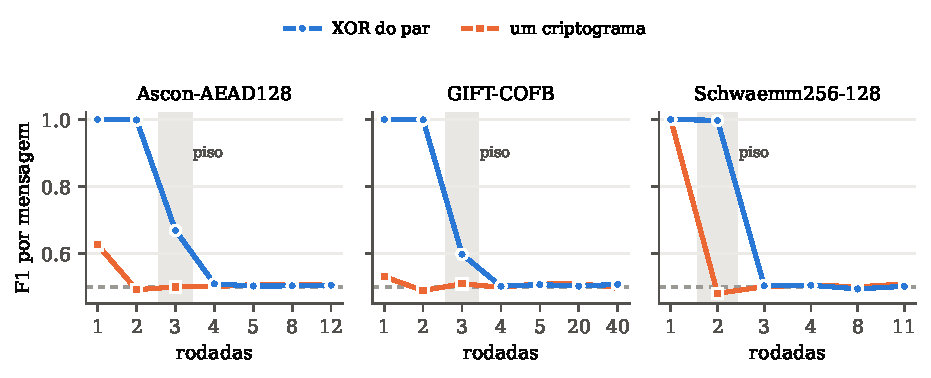
\includegraphics[width=\textwidth]{img/piso_f1_rodadas.pdf}
\caption{F1 por mensagem do melhor classificador, sem bolsa, por número de rodadas, com o XOR do par e com um criptograma isolado.}
\label{fig:res-piso}
\par\smallskip\footnotesize A faixa cinza marca o piso com o XOR do par, e a linha tracejada, o acaso.
\end{figure}

Uma única célula acima do piso merece menção. No Ascon-AEAD128 com quatro rodadas, o Random Forest sem bolsa teve F1 de 0,509, com o limite inferior do intervalo em 0,502, ligeiramente acima de 0,50. A célula ficou acima do teto da faixa de controle, mas não passou pela correção de Benjamini-Hochberg, e os outros dois classificadores na mesma condição ficaram em 0,495 e 0,507, de modo que a rodada não é contada como detectada.

A força do sinal no piso cresce quando o adversário junta várias mensagens do mesmo dispositivo. Por par, o Ascon-AEAD128 com três rodadas é reconhecido com F1 de 0,669 e o GIFT-COFB com três rodadas, com 0,598; com bolsas de 100 pares, esses valores sobem para 0,899 e 0,933. Um sinal fraco em cada mensagem se torna, para um adversário que escuta 200 mensagens de um dispositivo, uma decisão correta em cerca de nove de cada dez dispositivos.

Comparado com o criptograma isolado da Seção~\ref{sec:res-isolado}, que só denunciava a primeira rodada no Ascon-AEAD128 e no GIFT-COFB, o par leva o piso desses dois algoritmos de uma para três rodadas. No Schwaemm256-128, o piso já era 2 com o criptograma isolado, mas detectado em uma única célula, com o par, a mesma rodada é detectada nas nove, com F1 próximo de 1.

Em relação aos dois criptogramas lado a lado, o XOR não mudou o piso, mas tornou a rodada do piso detectável em mais células, nove e oito de nove no Ascon-AEAD128 e no GIFT-COFB, contra três, e nove de nove no Schwaemm256-128, contra sete. No Ascon-AEAD128 com três rodadas, o melhor F1 por par subiu de 0,554 para 0,669. O XOR, portanto, não cria o sinal, ele entrega ao classificador a comparação bit a bit entre as duas mensagens, que, sem ele, o classificador precisa aprender sozinho. A Tabela~\ref{tab:res-representacao} reúne os três passos e mostra que a fonte do sinal é observar duas mensagens da mesma chave.

\begin{table}[htb]
\centering
\caption{Piso e força do sinal conforme a representação apresentada ao classificador.}
\label{tab:res-representacao}
\footnotesize
\setlength{\tabcolsep}{4pt}
\begin{tabular}{llcccc}
\toprule
Algoritmo & Representação & Piso & Detectadas & F1, bolsa 1 & F1, bolsa 100 \\
\midrule
Ascon-AEAD128   & um criptograma & 1 & 0 de 9 & 0,500 & 0,583 \\
                & lado a lado    & 3 & 3 de 9 & 0,554 & 0,908 \\
                & XOR do par     & 3 & 9 de 9 & 0,669 & 0,899 \\
\midrule
GIFT-COFB       & um criptograma & 1 & 0 de 9 & 0,510 & 0,557 \\
                & lado a lado    & 3 & 3 de 9 & 0,516 & 0,625 \\
                & XOR do par     & 3 & 8 de 9 & 0,598 & 0,933 \\
\midrule
Schwaemm256-128 & um criptograma & 2 & 1 de 9 & 0,481 & 0,621 \\
                & lado a lado    & 2 & 7 de 9 & 0,987 & 1,000 \\
                & XOR do par     & 2 & 9 de 9 & 0,998 & 1,000 \\
\bottomrule
\end{tabular}
\par\smallskip\footnotesize Detectadas, F1, bolsa 1 e F1, bolsa 100 referem-se à rodada do piso com o XOR do par: três rodadas no Ascon-AEAD128 e no GIFT-COFB e duas no Schwaemm256-128.
\end{table}

\subsection{Piso de dados}
\label{sec:res-piso-dados}

O piso de rodadas diz até quantas rodadas o algoritmo reduzido é distinguível de dados aleatórios, mas não diz quanto dado o adversário precisa para fazer essa distinção. Esta subseção mede essa quantidade, que aqui se chama de piso de dados, em duas partes, o menor número de pares que o adversário precisa gerar, com chaves próprias, para treinar o classificador, e o menor número de pares que ele precisa observar do dispositivo-alvo para decidir. Para medir as duas, os três classificadores foram treinados, na rodada do piso, com conjuntos cada vez menores, de 30\,000 pares por classe até um único par, e avaliados nos mesmos 1\,000 dispositivos de teste, com bolsas de 1, 10 e 100 pares observados.

Cada parte tem dois níveis, o de detectar o sinal e o de decidir com confiança sobre um dispositivo. Detectar quer dizer que o classificador acerta mais que o acaso no conjunto dos 1\,000 dispositivos de teste, o que pode acontecer mesmo quando a decisão sobre cada dispositivo é pouco melhor que jogar uma moeda. Decidir com confiança quer dizer acertar a maior parte dos dispositivos, e aqui se toma como referência um F1 de 0,9, ou seja, cerca de nove acertos em cada dez dispositivos.

Quanto aos pares observados, com bolsas de um par, ou seja, quando o classificador decide a partir de um único par de mensagens de cada dispositivo, sem combinar a resposta com a de outros pares, o F1 sobre os 1\,000 dispositivos de teste já fica acima do acaso nos três algoritmos, desde que o treinamento seja suficiente, mas só no Schwaemm256-128 essa decisão é confiável. Com 30\,000 pares de treinamento, a bolsa de um par dá F1 de 0,999 no Schwaemm256-128 com duas rodadas, contra 0,679 no Ascon-AEAD128 e 0,608 no GIFT-COFB com três rodadas (Tabela~\ref{tab:res-dados-bolsa}). Nesses dois algoritmos, a decisão só passa de 0,9 com bolsas de 100 pares, ou 200 mensagens observadas, com F1 de 0,937 e 0,915.

Quanto ao treinamento, a Tabela~\ref{tab:res-dados-minimos} traz o menor número de pares com que cada classificador detecta o piso com bolsas de um par. No Schwaemm256-128 com duas rodadas, a regressão logística e o Random Forest detectam o piso com um único par de treinamento, e, com 20 pares, a regressão logística chega a F1 de 0,871 e o Random Forest a 0,969. No Ascon-AEAD128 com três rodadas, a regressão logística também passa pelo critério com um par de treinamento, mas com F1 de 0,507, no limite do que o critério aceita, e os três classificadores detectam a partir de 50 pares. O GIFT-COFB com três rodadas é o que exige mais dados, de 700 pares no XGBoost a 2\,000 no Random Forest. Nesses mínimos, porém, o classificador fica perto do acaso, e, para decidir com confiança, o Ascon-AEAD128 e o GIFT-COFB precisam de muito mais treinamento. Com bolsas de 100 pares, o F1 do Ascon-AEAD128 passa de 0,688 com 300 pares de treinamento para 0,888 com 3\,000 e 0,901 com 10\,000, e o do GIFT-COFB passa de 0,616 com 3\,000 para 0,884 com 10\,000 e 0,915 com 30\,000. No Schwaemm256-128, dois pares de treinamento já dão F1 de 0,992 com bolsas de 100 pares. Nenhuma das 504 células do braço aleatório foi detectada.

Na rodada do piso, portanto, o sinal já aparece no conjunto de teste com bolsas de um par e de 1 a 2\,000 pares de treinamento, conforme o algoritmo e o classificador, mas, com esses mínimos, a decisão sobre cada dispositivo fica perto do acaso. Para decidir com confiança sobre um dispositivo, ele sobe para cerca de 100 pares observados e de 10\,000 a 30\,000 pares de treinamento no Ascon-AEAD128 e no GIFT-COFB, enquanto no Schwaemm256-128 poucos pares bastam para as duas coisas.

\begin{table}[htb]
\centering
\caption{Menor treinamento com que cada classificador detecta a rodada do piso, com bolsas de um par.}
\label{tab:res-dados-minimos}
\footnotesize
\setlength{\tabcolsep}{4pt}
\begin{tabular}{lcccccc}
\toprule
 & \multicolumn{2}{c}{Regressão logística} & \multicolumn{2}{c}{Random Forest} & \multicolumn{2}{c}{XGBoost} \\
\cmidrule(lr){2-3}\cmidrule(lr){4-5}\cmidrule(lr){6-7}
Algoritmo & pares & F1 & pares & F1 & pares & F1 \\
\midrule
Ascon-AEAD128 (3 rodadas)   & 1     & 0,507 & 10    & 0,506 & 50  & 0,517 \\
GIFT-COFB (3 rodadas)       & 1\,000 & 0,504 & 2\,000 & 0,505 & 700 & 0,503 \\
Schwaemm256-128 (2 rodadas) & 1     & 0,572 & 1     & 0,562 & 10  & 0,605 \\
\bottomrule
\end{tabular}
\par\smallskip\footnotesize Pares: menor número de pares de treinamento por classe a partir do qual todos os níveis maiores testados também foram detectados. F1: F1 por par nesse nível. Níveis testados: 1, 2, 5, 10, 20, 50, 100, 200 e 300 pares no Ascon-AEAD128 e no Schwaemm256-128, e de 300 a 5\,000 pares no GIFT-COFB.
\end{table}

\begin{table}[htb]
\centering
\caption{Maior F1 entre os três classificadores na rodada do piso, por quantidade de treinamento e tamanho da bolsa.}
\label{tab:res-dados-bolsa}
\footnotesize
\setlength{\tabcolsep}{4pt}
\begin{tabular}{lcccc}
\toprule
Algoritmo & Pares de treinamento & Bolsa de 1 & Bolsa de 10 & Bolsa de 100 \\
\midrule
Ascon-AEAD128 (3 rodadas)   & 300     & 0,596 & 0,665 & 0,688 \\
                            & 1\,000  & 0,634 & 0,762 & 0,788 \\
                            & 3\,000  & 0,657 & 0,829 & 0,888 \\
                            & 10\,000 & 0,667 & 0,847 & 0,901 \\
                            & 30\,000 & 0,679 & 0,872 & 0,937 \\
\midrule
GIFT-COFB (3 rodadas)       & 300     & 0,500 & 0,504 & 0,504 \\
                            & 1\,000  & 0,505 & 0,516 & 0,547 \\
                            & 3\,000  & 0,513 & 0,536 & 0,616 \\
                            & 10\,000 & 0,571 & 0,705 & 0,884 \\
                            & 30\,000 & 0,608 & 0,776 & 0,915 \\
\midrule
Schwaemm256-128 (2 rodadas) & 300     & 0,992 & 1,000 & 1,000 \\
                            & 30\,000 & 0,999 & 1,000 & 1,000 \\
\bottomrule
\end{tabular}
\par\smallskip\footnotesize Treinamento com 3, 10, 30, 100 e 300 dispositivos de 100 pares cada, e teste nos mesmos 1\,000 dispositivos. No Schwaemm256-128, os níveis intermediários ficaram entre esses dois valores.
\end{table}

A Seção~\ref{sec:res-robustez} verifica se esse piso muda quando se altera a forma de medir.


\section{Robustez do piso}
\label{sec:res-robustez}

Esta seção verifica se o piso da Seção~\ref{sec:res-piso} depende das escolhas feitas para medi-lo. Foram variados, um de cada vez, a fase do algoritmo que é reduzida, a quantidade de dados de treinamento, os modelos e seus hiperparâmetros, o nonce e a fonte do texto em claro. Nenhuma dessas variações aumentou o piso de nenhum algoritmo, com uma exceção marginal, descrita a seguir (Tabela~\ref{tab:res-robustez}). A maioria o manteve, a posição do contador o reduziu em dois algoritmos, e algumas mudaram a força com que a rodada do piso é detectada, o que cada subseção discute.

\begin{table}[htb]
\centering
\caption{Piso de rodadas sob cada variação do experimento.}
\label{tab:res-robustez}
\footnotesize
\setlength{\tabcolsep}{4pt}
\begin{tabular}{lccc}
\toprule
Variação & Ascon-AEAD128 & GIFT-COFB & Schwaemm256-128 \\
\midrule
Experimento principal (Seção~\ref{sec:res-piso}) & 3 & 3 & 2 \\
Só a inicialização e a finalização reduzidas & 3 & não se aplica & 2 \\
Só as rodadas entre blocos reduzidas & nenhum & não se aplica & nenhum \\
Sem a tag (só o texto cifrado) & 3 & 3 & 2 \\
10 vezes mais dados & 3 & 3 & 2 \\
Hiperparâmetros ajustados, com SVM & 3 & 3 & 2 \\
MLP e CNN 1D, 10 vezes mais dados & 3 & 3 (só a MLP) & 2 \\
Contador no início do nonce & 3 & 2 & 1 \\
Corpus original (HTML e outros idiomas) & 3 & 3 & 2 \\
20\% das mensagens como imagens$^{*}$ & 3 (4$^{*}$) & 3 & 2 \\
\bottomrule
\end{tabular}
\par\smallskip\footnotesize $^{*}$Medido só na rodada do piso, na seguinte e na da especificação. No Ascon-AEAD128 com quatro rodadas, uma das nove células passou pelo critério.
\end{table}

O estudo principal usa livros em inglês, sem marcação. Com o corpus original, que inclui marcação HTML e livros em outros idiomas, os pisos foram os mesmos, e o melhor F1 por par na rodada do piso foi de 0,650 no Ascon-AEAD128, 0,566 no GIFT-COFB e 0,989 no Schwaemm256-128, contra 0,669, 0,598 e 0,998 no estudo principal. Para verificar se uma fonte com outra estrutura reduziria o piso, o estudo foi repetido com 20\% das mensagens trocadas por imagens, só na rodada do piso, na seguinte e na da especificação. O piso não diminuiu em nenhum algoritmo, mas o sinal ficou mais fraco, com F1 por par de 0,600, 0,547 e 0,959 na rodada do piso. Com bolsas de 100 pares, o F1 ficou em 0,882, 0,832 e 1,000, contra 0,899, 0,933 e 1,000 no estudo principal. No Ascon-AEAD128 com quatro rodadas, uma das nove células passou pelo critério, com o Random Forest, bolsas de um par e F1 de 0,512, enquanto as outras oito ficaram no acaso.

\subsection{Diferenças entre inicialização e rodadas entre blocos}
\label{sec:res-fase}

No Ascon-AEAD128 e no Schwaemm256-128, as rodadas de inicialização e as rodadas entre blocos foram reduzidas juntas no experimento principal. Para saber qual das duas fases responde pelo piso, cada uma foi reduzida separadamente, com a outra mantida na especificação (Tabela~\ref{tab:res-fase}). Com só a inicialização e a finalização reduzidas, o piso e a força do sinal foram praticamente iguais aos do experimento principal: no Ascon-AEAD128 com três rodadas, nove de nove células detectadas e F1 de 0,667 por par, contra 0,669, e no Schwaemm256-128 com duas rodadas, nove de nove células e F1 de 0,998. Com só as rodadas entre blocos reduzidas, nenhuma das 72 células do Ascon-AEAD128, de uma a oito rodadas, e nenhuma das 63 do Schwaemm256-128, de uma a sete, foi detectada, nem com uma única rodada entre blocos. O sinal persistiu, portanto, quando a redução ficou restrita à inicialização e à finalização, e desapareceu quando ficou restrita às rodadas entre blocos. Como a finalização produz a tag, que também entra na amostra, essa comparação sozinha não separa a inicialização da finalização. Para separá-las, os dois estudos foram refeitos sem a tag, só com os 64 bytes de texto cifrado, que dependem da inicialização e das rodadas entre blocos, mas não da finalização, que só acontece depois do último bloco. Sem a tag, o piso e a força do sinal foram os mesmos. Com as duas fases reduzidas, o melhor F1 por par na rodada do piso foi de 0,671 no Ascon-AEAD128, 0,595 no GIFT-COFB e 0,998 no Schwaemm256-128, e, com só a inicialização e a finalização reduzidas, de 0,670 no Ascon-AEAD128 e 0,998 no Schwaemm256-128. Como o texto cifrado não passa pela finalização, a hipótese mais forte é que o sinal que define o piso venha da inicialização, mas ela não foi testada diretamente, já que nenhum estudo reduziu só a inicialização, com a finalização completa. O GIFT-COFB não entra nesta comparação, porque usa o mesmo número de rodadas em todas as chamadas da cifra de bloco.

\begin{table}[htb]
\centering
\caption{Piso de rodadas conforme a fase do algoritmo que é reduzida.}
\label{tab:res-fase}
\footnotesize
\setlength{\tabcolsep}{3pt}
\begin{tabular}{llccccc}
\toprule
Algoritmo & Fase reduzida & Piso & Detectadas & F1, bolsa 1 & F1, bolsa 100 & Seguinte \\
\midrule
Ascon-AEAD128   & as duas & 3 & 9 de 9 & 0,669 & 0,899 & 0 de 9 \\
                & inicialização e finalização & 3 & 9 de 9 & 0,667 & 0,925 & 0 de 9 \\
                & entre blocos & nenhum & \multicolumn{4}{c}{0 de 72 células (1 a 8 rodadas)} \\
\midrule
Schwaemm256-128 & as duas & 2 & 9 de 9 & 0,998 & 1,000 & 0 de 9 \\
                & inicialização e finalização & 2 & 9 de 9 & 0,998 & 1,000 & 0 de 9 \\
                & entre blocos & nenhum & \multicolumn{4}{c}{0 de 63 células (1 a 7 rodadas)} \\
\bottomrule
\end{tabular}
\par\smallskip\footnotesize Fase reduzida: as duas é o experimento principal; nas outras linhas, a fase não reduzida fica na especificação. Detectadas e Seguinte: células detectadas, entre as nove, na rodada do piso e na rodada seguinte. F1: maiores valores entre os três classificadores na rodada do piso.
\end{table}

\subsection{Quantidade de dados}
\label{sec:res-dados}

Para verificar se a rodada seguinte ao piso deixa de parecer aleatória quando há mais dados, a regressão logística foi treinada com 1 e 10 vezes a quantidade do experimento principal, 300 e 3\,000 dispositivos com 100 pares cada, ou seja, 30 mil e 300 mil pares, e avaliada sempre nos mesmos 1\,000 dispositivos de teste. Na rodada seguinte ao piso, o F1 por par ficou entre 0,499 e 0,501 nas duas quantidades de dados, nos três algoritmos. Na rodada do piso, o ganho foi pequeno: no Ascon-AEAD128 com três rodadas, o F1 por par passou de 0,661 para 0,665, e no Schwaemm256-128 com duas rodadas, de 0,946 para 0,947. O GIFT-COFB foi o que mais ganhou, de 0,524 para 0,533 por par e de 0,692 para 0,735 com bolsas de 100 pares, e ainda assim a rodada seguinte não saiu do acaso. Até os volumes testados, portanto, mais dados não produziram detecção acima do piso com esse detector.

\subsection{Modelos e hiperparâmetros}
\label{sec:res-modelos}

Os classificadores do experimento principal usaram configurações fixas, definidas antes dos experimentos. Para verificar se um ajuste de hiperparâmetros mudaria o piso, foi feita uma busca de hiperparâmetros com o teste separado, e a configuração de cada classificador foi escolhida apenas com as chaves de treinamento, por validação cruzada de três dobras separadas por chave, na rodada seguinte ao piso, que é onde um ganho mudaria o resultado, e a configuração escolhida foi avaliada uma única vez no teste. Foram buscadas seis configurações da regressão logística, vinte do Random Forest e vinte do XGBoost (Tabela~\ref{tab:res-hiperparametros}). O SVM com núcleo RBF não entrou no experimento principal por custo computacional: o seu tempo de ajuste cresce com cerca de $n^{2{,}5}$, e, com as 38 a 48 mil amostras de treinamento de cada configuração, cada ajuste levaria de 14 a 25 minutos, contra cerca de 10 segundos do Random Forest. Ele entrou nesta busca com nove configurações, avaliadas numa subamostra de 8\,000 exemplos. Na rodada seguinte ao piso, a AUC de validação de todas as configurações, nos três algoritmos, ficou entre 0,478 e 0,506, e com as configurações escolhidas os pisos foram os mesmos: 3, 3 e 2.

\begin{table}[htb]
\centering
\caption{Espaço da busca de hiperparâmetros e configuração escolhida em cada algoritmo.}
\label{tab:res-hiperparametros}
\footnotesize
\setlength{\tabcolsep}{2pt}
\begin{tabular}{lllcccc}
\toprule
Classificador & Hiperparâmetro & Valores avaliados & Principal & Ascon & GIFT & Schwaemm \\
\midrule
Reg. logística & $C$ & $10^{-3}$, $10^{-2}$, $10^{-1}$, 1, 10, 100 & 1 & $10^{-3}$ & 10 & $10^{-3}$ \\
\midrule
Random Forest & árvores & 200, 500, 1\,000 & 500 & 500 & 500 & 200 \\
(20 sorteios) & bits por divisão & $\sqrt{n}$, 10\%, 30\% & $\sqrt{n}$ & $\sqrt{n}$ & $\sqrt{n}$ & 10\% \\
 & folha mínima & 1, 5, 20 & 1 & 5 & 5 & 1 \\
 & profundidade máxima & sem limite, 12, 24 & sem limite & 12 & 12 & 24 \\
\midrule
XGBoost & árvores & 200, 500, 1\,000, 2\,000 & 500 & 200 & 200 & 200 \\
(20 sorteios) & profundidade máxima & 3, 6, 9, 12 & 6 & 12 & 3 & 12 \\
 & taxa de aprendizado & 0,01, 0,03, 0,1, 0,3 & 0,1 & 0,1 & 0,1 & 0,1 \\
 & fração de exemplos & 0,6, 0,8, 1 & 1 & 0,8 & 1 & 0,8 \\
 & fração de bits & 0,3, 0,6, 1 & 1 & 0,3 & 0,3 & 0,3 \\
\midrule
SVM RBF & $C$ & 0,1, 1, 10 & não usado & 10 & 1 & 10 \\
(grade) & $\gamma$ & $0{,}1/n$, $1/n$, $10/n$ & não usado & $0{,}1/n$ & $0{,}1/n$ & $0{,}1/n$ \\
\bottomrule
\end{tabular}
\par\smallskip\footnotesize $n$: número de variáveis da amostra, 640 bits. Principal: configuração do estudo principal (Seção~\ref{sec:met-classificadores}). Ascon, GIFT e Schwaemm: configuração escolhida pela validação cruzada na rodada seguinte ao piso, aplicada depois às rodadas do piso, à seguinte e à da especificação, nos dois braços. Como todas as configurações ficaram no acaso nessa rodada, a escolha entre elas não reflete um ganho real.
\end{table}

Também foram avaliadas duas redes neurais, treinadas com 10 vezes os dados do experimento principal: uma rede densa (MLP) e uma rede convolucional unidimensional sobre os bytes (CNN 1D), nas rodadas 1, do piso, seguinte ao piso e da especificação. As duas detectaram a rodada do piso no Ascon-AEAD128 e no Schwaemm256-128 e não detectaram a rodada seguinte. No GIFT-COFB com três rodadas, a MLP teve F1 de 0,553 por par, acima dos 0,533 da regressão logística da Seção~\ref{sec:res-dados}, com a mesma quantidade de dados, enquanto a CNN 1D não detectou essa rodada, porque passou a prever quase sempre a mesma classe. No Ascon-AEAD128 com três rodadas, ao contrário, as redes ficaram abaixo da regressão logística, com 0,621 e 0,642, contra 0,665. Em nenhum algoritmo uma rede detectou a rodada seguinte ao piso.

\subsection{Posição do contador no nonce}
\label{sec:res-contador}

No experimento principal, o contador ocupa os últimos bytes do nonce. Como a posição em que a diferença entre os dois nonces entra no algoritmo pode influenciar o quanto ela se espalha, o experimento foi repetido nos três algoritmos com o contador nos primeiros bytes. No Ascon-AEAD128, o piso continuou em três rodadas, com a rodada 4 sem detecção nas nove células, mas a rodada 3 ficou muito mais forte, com F1 de 0,893 por par, contra 0,669 com o contador no fim. No GIFT-COFB e no Schwaemm256-128, o efeito foi o oposto, e o piso caiu uma rodada, para 2 e para 1. No GIFT-COFB com duas rodadas, o F1 por par passou de 0,999 para 0,878, e a rodada 3 deixou de ser detectada; no Schwaemm256-128, a rodada 2, que tinha F1 de 0,998 com o contador no fim, passou a ficar no acaso. A posição do contador muda, portanto, o piso, mas em nenhum algoritmo o contador no início produziu um piso maior que o contador no fim, de modo que o piso do experimento principal é o maior entre as duas posições testadas.

O contador começando do zero corresponde a um dispositivo recém-ligado. Para o caso em que o contador de cada dispositivo está num ponto qualquer, o experimento foi repetido com o contador começando de um valor sorteado por dispositivo, com o corpus original, que inclui marcação HTML, e não com os livros em inglês do estudo principal. Com essa fonte, o contador começando do zero deu os mesmos pisos do estudo principal. Com o contador sorteado, o Ascon-AEAD128 e o Schwaemm256-128 mantiveram o piso, e o GIFT-COFB caiu uma rodada, para 2.

No estudo principal, o par é formado por duas mensagens consecutivas, com nonces $2j$ e $2j+1$, que diferem em um único bit. Para verificar se o par precisa ser consecutivo, o estudo foi repetido com pares de nonces $c$ e $c+k$, com $k$ entre 2 e 256 e $c$ múltiplo de $2k$, para que nenhum nonce se repita no mesmo dispositivo. Com $k$ potência de 2, os dois nonces continuam diferindo em um único bit, numa posição mais alta do contador, e, com $k$ igual a 3, 7 ou 15, a diferença tem vários bits, de três a quatro e meio em média, dependendo do par (Tabela~\ref{tab:res-distancia}). Quando os nonces diferem em um único bit, o piso foi o mesmo das mensagens consecutivas nos três algoritmos, mesmo com as mensagens a 256 posições de distância, e só a força do sinal mudou, conforme o bit, com o F1 por par do Ascon-AEAD128 com três rodadas entre 0,650 e 0,836. Quando a diferença tem vários bits, o F1 caiu. O GIFT-COFB perdeu uma rodada nos três casos, e o Ascon-AEAD128 com $k$ igual a 7 e 15, enquanto o Schwaemm256-128 manteve o piso de dois passos, com F1 por par de 0,997 ou mais em todas as distâncias. O piso depende, portanto, de quantos bits separam os dois nonces, e não da distância entre as mensagens, e, como os nonces são públicos, o adversário pode escolher no tráfego os pares que diferem em um único bit. No braço aleatório, nenhuma distância produziu piso, e 6 das 1\,620 células foram detectadas, todas com a tag incluída.

\begin{table}[htb]
\centering
\caption{Piso e F1 por par com nonces a distância $k$.}
\label{tab:res-distancia}
\small
\setlength{\tabcolsep}{4pt}
\begin{tabular}{rcccccc}
\toprule
 & & \multicolumn{2}{c}{Ascon-AEAD128} & \multicolumn{2}{c}{GIFT-COFB} & Schwaemm256-128 \\
\cmidrule(lr){3-4}\cmidrule(lr){5-6}\cmidrule(lr){7-7}
$k$ & bits de diferença & piso & F1 com 3 & piso & F1 com 3 & piso (F1 com 2) \\
\midrule
1   & 1 & 3 & 0,669 & 3 & 0,598 & 2 (0,998) \\
2   & 1 & 3 & 0,797 & 3 & 0,515 & 2 (0,997) \\
4   & 1 & 3 & 0,668 & 3 & 0,603 & 2 (0,997) \\
8   & 1 & 3 & 0,836 & 3 & 0,588 & 2 (0,998) \\
16  & 1 & 3 & 0,650 & 3 & 0,595 & 2 (0,997) \\
64  & 1 & 3 & 0,671 & 3 & 0,580 & 2 (0,997) \\
256 & 1 & 3 & 0,678 & 3 & 0,576 & 2 (0,997) \\
\midrule
3   & 2 a 10 (média 3,0) & 3 & 0,552 & 2 & 0,503 & 2 (0,997) \\
7   & 3 a 10 (média 4,0) & 2 & 0,505 & 2 & 0,503 & 2 (0,997) \\
15  & 3 a 12 (média 4,5) & 2 & 0,510 & 2 & 0,505 & 2 (0,998) \\
\bottomrule
\end{tabular}
\par\smallskip\footnotesize O F1 é o melhor F1 por par entre os três classificadores, com bolsas de um par, na rodada do piso do estudo principal. $k=1$ é o estudo principal.
\end{table}


\section{Síntese}
\label{sec:res-sintese}

A Tabela~\ref{tab:res-sintese} reúne os pisos medidos neste capítulo. Com criptogramas de 64~KB descritos por atributos estatísticos, nenhum algoritmo foi distinguido, nem com uma rodada. Com um criptograma isolado de 80 bytes, os três algoritmos só foram separados de dados aleatórios praticamente sem rodadas: com uma rodada no Ascon-AEAD128 e no GIFT-COFB, e com duas, de forma marginal, no Schwaemm256-128. Observando duas mensagens consecutivas do mesmo dispositivo, o piso subiu para 3 das 12 rodadas no Ascon-AEAD128 e para 3 das 40 no GIFT-COFB, e a rodada 2 do Schwaemm256-128 passou a ser detectada com F1 próximo de 1. Na rodada do piso, com bolsas de um par, em que cada decisão usa um único par de mensagens, o F1 sobre o conjunto de teste já fica acima do acaso, mas, no Ascon-AEAD128 e no GIFT-COFB, decidir sobre um dispositivo com F1 de pelo menos 0,9 exige bolsas de cerca de 100 pares.

\begin{table}[htb]
\centering
\caption{Pisos de rodadas medidos no capítulo.}
\label{tab:res-sintese}
\footnotesize
\setlength{\tabcolsep}{4pt}
\begin{tabular}{lccc}
\toprule
Algoritmo & Especificação & Isolado, 80 bytes & Par de mensagens \\
\midrule
Ascon-AEAD128   & 12 & 1 & 3 \\
GIFT-COFB       & 40 & 1 & 3 \\
Schwaemm256-128 & 11 & 2 & 2 \\
\bottomrule
\end{tabular}
\end{table}

A progressão da Seção~\ref{sec:res-piso} e as verificações da Seção~\ref{sec:res-robustez} mostram de onde vem esse piso e o que não o altera. O sinal vem de observar duas mensagens da mesma chave, e não do XOR, que apenas o torna mais fácil de aprender, e persistiu quando a redução ficou restrita à inicialização e à finalização, inclusive sem a tag, que é produzida pela finalização, enquanto reduzir só as rodadas entre blocos não produziu piso nenhum. A hipótese mais forte é, portanto, que o sinal que define o piso venha da inicialização. Até os volumes e os modelos testados, mais dados de treinamento, hiperparâmetros ajustados e redes neurais não subiram o piso de nenhum algoritmo. A posição do contador no nonce pode reduzir o piso, mas, entre as posições testadas, o contador no fim foi sempre a mais favorável ao adversário.

Esses são os resultados observados, e as explicações para eles ficam para o Capítulo~\ref{cap:discussao}. Em todos os casos, o piso é um limite do instrumento nas condições testadas, e não uma prova de segurança acima dele. Até aquele número de rodadas, o algoritmo reduzido é distinguível de dados aleatórios por um adversário que só observa os criptogramas; acima dele, a ausência de detecção indica apenas que os detectores avaliados, com a quantidade de dados usada, não separam. O Capítulo~\ref{cap:discussao} discute as explicações propostas para esses resultados e os compara com a literatura.
